\section{Synthesis} % (fold)
For the hardware implementation of the project Vivado software by Xilinx was used. This software enabled to map the VHDL code on Zynq-7000 board. To reach the final implementation and discover the maximum operating frequency the typical flow of Vivado was followed i.e. from VHDL code to RTL analysis, synthesis and as last implementation.
\label{sec:synthesis_and_implementation}
\subsection{RTL Design}
\begin{figure}[H]
  \centering
  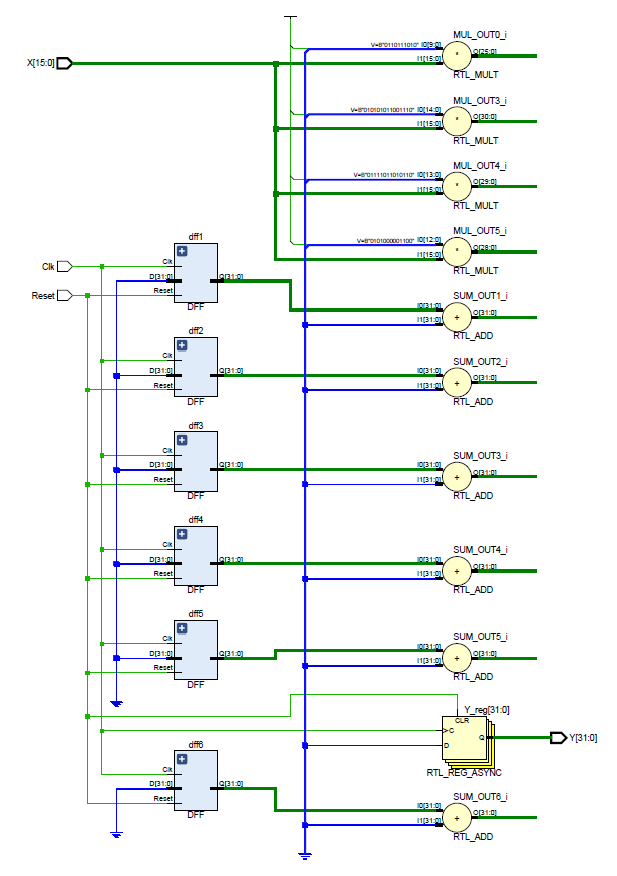
\includegraphics[width=0.9\linewidth]{./images/schematic.PNG}
  \caption{RTL design from vivado}
  \label{fig:schematic}
\end{figure}
\subsection{Synthesis}
A clock period of 10 ns was set. The synthesis was carried without any kind of warnings displayed.\\
\textbf{Timing report} Timing report is fine and states that all constraints are met:
\begin{figure}[H]
  \centering
  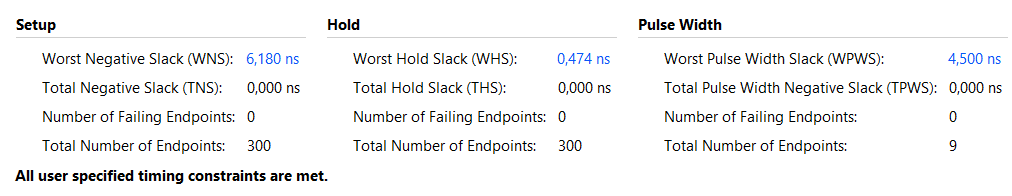
\includegraphics[width=0.9\linewidth]{./images/timing.PNG}
  \caption{Timing summary from vivado}
  \label{fig:timing}
\end{figure}
\textbf{Power report} 
\begin{figure}[H]
  \centering
  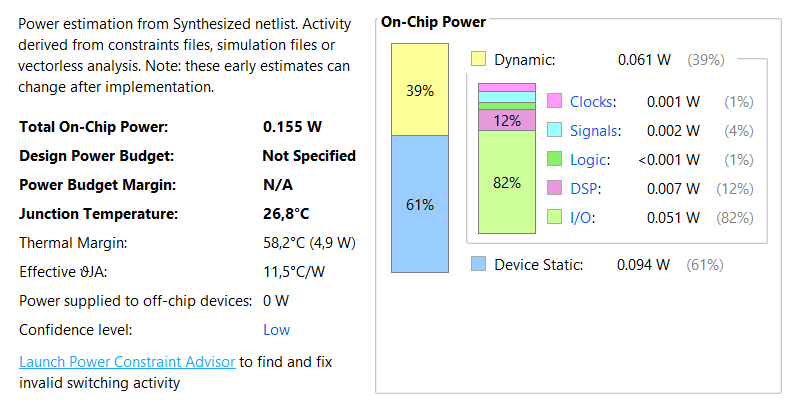
\includegraphics[width=0.9\linewidth]{./images/power.PNG}
  \caption{Power summary from vivado}
  \label{fig:power}
\end{figure}
\textbf{Utilization report}

\begin{figure}[H]
  \centering
  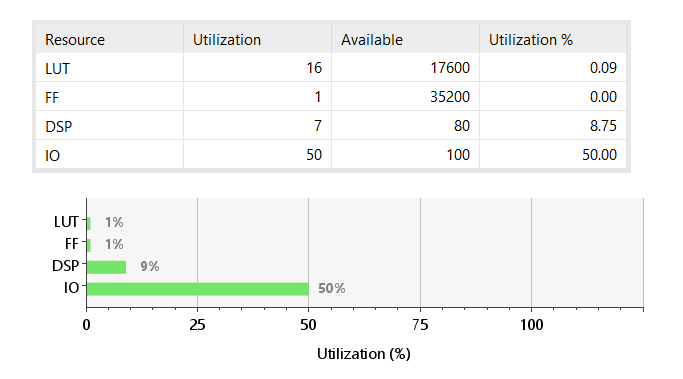
\includegraphics[width=0.9\linewidth]{./images/utilization.PNG}
  \caption{Utilization summary from vivado}
  \label{fig:utilization}
\end{figure}
\ref{fig:utilization} shows how the most widely used resource is the I/O this derives from the fact that the circuit has 16 bit inputs and a 32 bit output.
\subsection{Critical path} % (fold)
\label{sub:critical_path}
Vivado shows how the critical path includes the sum and multiplication operation from the output of a registry till the input to the next registry.
\begin{figure}[H]
  \centering
  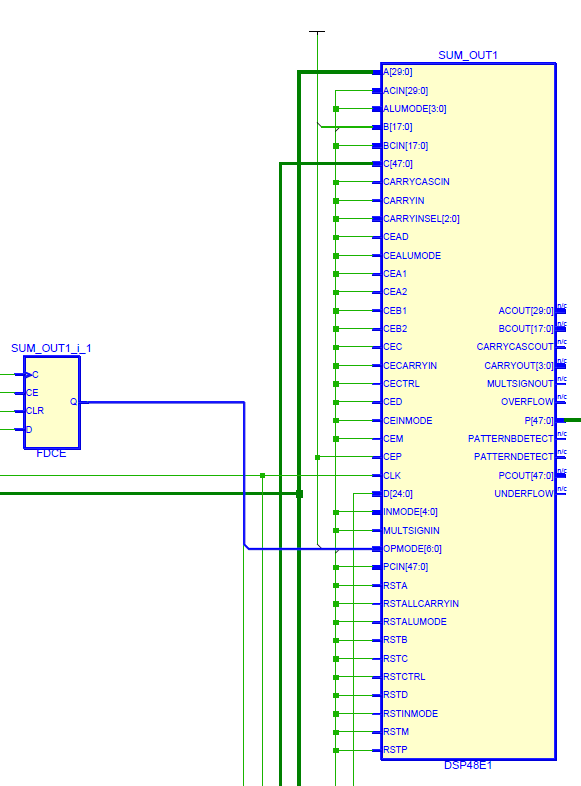
\includegraphics[width=0.9\linewidth]{./images/critical}
  \caption{Critical path highlighted by vivado}
  \label{fig:critical}
\end{figure}
\subsection{Maximum operating frequency} % (fold)
\label{sub:maximum_operating_frequency}
From the timing report a positive Worst Negative Slack suggests that the circuit is not operating at the maximum frequency possible.
\begin{equation}
	f_{max} = \frac{1}{t_{clk}-slack}=\frac{1}{10ns-6.18ns}= \frac{1}{3.82ns}= 260 Mhz
	\label{eq:fmax}
\end{equation}
Equation \ref{eq:fmax} states that the maximum frequency at which the clock can be guided is 260 Mhz.
% subsection maximum_operating_frequency (end)

% subsection critical_path (end)
\section{Implementation}
The implementation was carried out without any warning. The data reported by the implementation confirm the conclusion derived in the synthesis step with slight differences such as the fact that the worst negative slack is now of $6.017ns$ hence the circuit has a maximum operating frequency of $251.1Mhz$ due to I/O ports being actually assigned and this brings some delay. 
